\documentclass[10pt]{article}

\usepackage[margin=1in]{geometry}
\usepackage{amsmath,amssymb}
\usepackage{booktabs}
\usepackage{graphicx}
\usepackage{array}
\usepackage[hidelinks]{hyperref}

\setlength{\parskip}{0.15em}
\newcolumntype{L}[1]{>{\raggedright\arraybackslash}p{#1}}

% Let floats fill more of a page, so tables do not push text onto pages of
% their own.
\renewcommand{\topfraction}{0.92}
\renewcommand{\bottomfraction}{0.85}
\renewcommand{\textfraction}{0.06}
\renewcommand{\floatpagefraction}{0.80}
\setlength{\textfloatsep}{12pt plus 2pt minus 3pt}
\setlength{\intextsep}{10pt plus 2pt minus 3pt}

\newcommand{\notes}[2]{\par\vspace{0.4em}%
  \begin{minipage}{#1}\footnotesize #2\end{minipage}}

\begin{document}

\begin{center}
{\Large\bfseries Housing First or Treatment First?}\\[0.35em]
{\large A stylized model}\\[0.35em]
\today
\end{center}
\vspace{0.8em}


%======================================================================
\section{Three questions}\label{sec:what}

In the data, drug use is concentrated among low income households, most of the
homeless do not carry a substance use disorder, and housing vouchers reach only
about a quarter of the households eligible for them. The quantitative model is
built to match facts of that kind, and it has six state variables and roughly
forty parameters, which is what the welfare and fiscal questions require but
makes it hard to see which piece of the environment does the work. This note
strips the environment to the smallest one in which three questions are still
well posed.

\begin{enumerate}\setlength{\itemsep}{0.25em}\setlength{\parskip}{0em}

\item \textbf{Who uses drugs?} Use is concentrated at the bottom of the income
distribution. Drugs are a normal good bought at a price, so that concentration
is not what a model produces by default. Which feature of the environment
reverses it, and can any other?

\item \textbf{What does housing assistance do to that decision?} A voucher pulls
drug use in two opposite directions. It raises the value of staying clean,
because a housed future is worth more than a homeless one and using puts that
future at risk: call this the value of life force, and it lowers use. It also
cushions the consequence of acquiring the disorder, because a household that
acquires one is housed anyway: call this the moral hazard force, and it raises
use. Both are first order, so theory does not sign the effect of housing
assistance on drug use, and the question is quantitative.

\item \textbf{When is Treatment First better than Housing First?} In the model
as it stands, never. There are no externalities from addiction and
homelessness, and so Housing First always raises welfare when agents are
forward looking, as they are here. Addiction creates a genuine tension, since
the same voucher that insures a household also makes the risk it insures more
attractive, but that tension alone cannot justify conditionality. However, if
addiction and homelessness generate an externality, such as reducing the
earning potential of children, then Treatment First may be preferred. The
model's work here is to show why the first claim holds and then to price the
externality that overturns it.

\end{enumerate}

The model is qualitative throughout: the calibration is rough by design, there is
no validation exercise, and every component has been removed and the model
refitted without it, so what remains is what the results need. The welfare
evaluations below are for illustration only; the full quantitative model is what
settles the main question.

%======================================================================
\section{The environment}\label{sec:env}

\subsection{Households and preferences}

There are three periods and a continuum of households. A period stands for
roughly twenty years of adult life. Survival, recovery and the unemployment
probabilities are per period numbers, while $\beta$ and $R$ take conventional
annual values rather than compounded ones, deliberately: compounding over
twenty years would leave the continuation value too small to matter, and
everything in Section~\ref{sec:who} runs through the continuation value.
Nothing below turns on the exact horizon, since every comparison varies one
object and holds the rest of the parameter vector fixed.

A household is characterised by its permanent income $y$, fixed over its life
and lognormally distributed, $\log y \sim \mathcal{N}(-\tfrac12\sigma^2,
\sigma^2)$, so mean income is one and every quantity below measured in units of
income is a multiple of the population average. Households differ in $y$ and in
nothing else, so every household at a given income makes the same choice and
drug use is a threshold in income rather than a probability. That also keeps
intact the paper's claim to generate the income gradient without ex ante
preference heterogeneity: there is none here to do the work.

Flow utility depends on non durable consumption $c$, the flow of housing
services $h$ consumed that period, and drug consumption $v$,
\begin{equation}\label{eq:u}
u(c,h,v) \;=\; (1-\gamma-\theta)\log c \;+\; \gamma \log h
\;+\; \theta\big[\log(b+v)-\log b\big] \;+\; \aleph .
\end{equation}
The three weights sum to one, so $\gamma$ is the housing budget share proper.
Housing services are chosen each period from the three point grid
$\{h_0,h_S,h_L\}$ of equation~\eqref{eq:opts}. The pair $(\theta,b)$ governs the
drug term: the marginal utility of the $v$th unit is $\theta/(b+v)$, so $\theta$
mostly sets how much a user uses and $b$ whether anyone uses at all. The Stone
and Geary form keeps the first unit's marginal utility finite, since under plain
$\theta\log v$ every household uses whatever the consequences. Finally $\aleph$
is the flow value of being alive, the utility of surviving into a period over
and above what is consumed in it: it gives mortality a cost that does not vanish
when consumption is low, and Section~\ref{sec:who} turns on it. Households
discount at $\beta$, save in one risk free asset at gross return $R$, and cannot
borrow.

\subsection{Timing}

\paragraph{Period 1.} Every household is employed and clean. It chooses
consumption, housing, drug use $v\ge0$ and saving, paying market rent on
whatever unit it picks. For simplicity, this is the only period in which it
chooses whether to use. Using generates the risk of a substance use disorder
next period, rising in $v$,
\begin{equation}\label{eq:hazard}
\pi(v) \;=\; 1 - e^{-\lambda v} .
\end{equation}
Because $\pi$ is increasing, the household internalises that using more is
riskier, so the intensive and extensive margins are not separate decisions.

\paragraph{Period 2.} For households that used, a disorder $d\in\{0,1\}$ is
realised with probability $\pi(v)$; for the rest it is not. Employment status
$\chi\in\{0,1\}$ is realised, with $\chi=1$ denoting unemployment, which occurs
with probability $u_0$, or the higher $u_1$ if $d=1$. An unemployed household
receives income support. It then chooses consumption, housing and saving. The
probability of recovering by the next period is $\rho$.

\paragraph{Period 3.} Terminal. Employment, income support, the voucher and the
housing choice work as in period 2, there is no drug use decision, and assets are
run down with nothing bequeathed.

\paragraph{Mortality, and why there are three periods.} A household survives from
one period to the next with probability
\begin{equation}\label{eq:surv}
\phi(d) \;=\; \phi_0\,(1-\kappa d),
\end{equation}
so $\kappa$ is the proportional reduction in survival caused by the disorder.
The third period is what makes that reduction bite. Mortality is a tax on a
continuation value, so it can only matter if there is a period after the one in
which the disorder is carried. In a two period version the disorder is realised
in the last period, death costs nothing because nothing follows it, and the
mechanism the whole model rests on is silent: recalibrated as a two period
model, the moral hazard of Section~\ref{sec:mh} collapses from $+3.57$
percentage points to $+0.23$. Three periods is the smallest number at which
acquiring the disorder has a future to destroy.

\subsection{Employment, income support and housing}\label{sec:support}

The gap $u_1-u_0$ is the entire resource cost of the disorder: there is no wage
penalty conditional on working, because the quantitative model sets that
parameter to one. Income in a period, given permanent income $y$ and employment
status $\chi$, is
\begin{equation}\label{eq:inc}
y_e(y,\chi) \;=\;
\begin{cases}
y & \text{if } \chi = 0,\\[0.2em]
\psi\cdot\min\{y,\bar y\} & \text{if } \chi = 1,
\end{cases}
\end{equation}
with $\psi$ the replacement rate and $\bar y$ a cap on the earnings base. There
is no other income risk. The quantitative model has persistent productivity
shocks as well, and they are not a key channel for anything asked here: what
links the disorder to housing is the loss of a job, not the ordinary
fluctuation of earnings around a trend.

The level of $\psi$ links the disorder to homelessness: for the poorest
households half of income falls short of the rent on the smallest unit, so an
unemployed household there cannot house itself out of current income, and were
income support above that rent the moral hazard of Section~\ref{sec:mh} would be
zero. The cap matters instead for Section~\ref{sec:who}: without it the resource
cost of the disorder would be exactly proportional to income, and a penalty
proportional to income cannot move a gradient that income itself generates.

Consumption is the numeraire, and the rent per unit of housing services $p_r$ is
normalised to one, so a unit's size and its market rent are the same number.
Each period the household chooses
\begin{equation}\label{eq:opts}
h \in \{h_0,\ h_S,\ h_L\}, \qquad h_0 < h_S < h_L ,
\end{equation}
homelessness, a small unit and a standard unit. Homelessness is free and
delivers almost nothing. Two rented sizes is the fewest that lets a household
economise on housing rather than lose it: with one, homelessness comes out at
$3.29$ per cent against a target of $0.40$, at any $h_0$.

A voucher covers part of the rent, is means tested and is rationed. Writing
$z\in\{0,1\}$ for whether one is held,
\begin{equation}\label{eq:vouch}
\Pr(z=1 \mid y_e, d) \;=\; \pi_V \cdot \mathbf{1}\{y_e \le y_V\}
\cdot \mathbf{1}\{\text{policy covers } d\},
\end{equation}
and a household holding one pays the fraction $\kappa_r$ of market rent, so the
rent paid on option $j$ is
\begin{equation}\label{eq:rent}
r_j(z) \;=\; p_r\,h_j\big[\kappa_r z + (1-z)\big]\cdot
\mathbf{1}\{j \ne 0\},
\end{equation}
which is zero when the household is homeless. Vouchers operate in periods 2 and
3. The parameter $\pi_V$ is the generosity of the programme and is the policy
dial of Section~\ref{sec:mh}.

The two policies differ in exactly one respect, the last indicator in
equation~\eqref{eq:vouch}. \textbf{Housing First} covers every eligible
household regardless of $d$. \textbf{Treatment First} covers only households
without the disorder. Since cover in the disorder state is the only difference,
the gap between them is the moral hazard and the whole of it.

\subsection{The household's problem}\label{sec:problem}

Solve backward, with $a$ assets carried in, $y$ permanent income, $\chi$
employment status, $z$ the voucher and $d$ the disorder, and write
$c_j = Ra + y_e(y,\chi) - r_j(z) - a'$ for consumption on housing option $j$. In
period 3 the household consumes everything, so $a'=0$, and chooses housing,
\begin{equation}\label{eq:v3}
\widetilde W_3(a,y,\chi,z) = \max_{j}
\big\{ (1-\gamma-\theta)\log c_j + \gamma \log h_j + \aleph \big\},
\end{equation}
and the value of entering period 3, taking expectations over employment and the
voucher lottery, both of which depend on $d$, is $W_3(a,y,d) = \mathbb{E}
[\widetilde W_3 \mid y, d]$. In period 2 the household also saves and faces
mortality and recovery,
\begin{equation}\label{eq:v2}
\widetilde W_2(a,y,\chi,z,d) = \max_{j,\,a'\ge0}
\big\{ (1-\gamma-\theta)\log c_j + \gamma \log h_j + \aleph
+ \beta\,\phi(d)\, \mathbb{E}_{d'} W_3(a',y,d') \big\},
\end{equation}
with $W_2(a,y,d) = \mathbb{E}[\widetilde W_2 \mid y,d]$ and $d'=0$ with
probability $\rho$ if $d=1$ and $d'=d$ otherwise. In period 1 the household is
employed, clean and holds no voucher, so $c_j = y - r_j(0) - p_v v - a'$, and it
chooses housing, drug use and saving,
\begin{equation}\label{eq:v1}
V_1(y) = \max_{j,\,v \ge 0,\,a' \ge 0}
\big\{ (1-\gamma-\theta)\log c_j + \gamma \log h_j
+ \theta[\log(b+v)-\log b] + \aleph
+ \beta\,\phi_0\, \mathbb{E}_{d'} W_2(a',y,d') \big\},
\end{equation}
where the disorder arrives with the use dependent probability
of~\eqref{eq:hazard}. Housing is a choice in period 1 as in every other period,
which is why $r_j(0)$ appears there: $y$ is income, not income net of an assumed
rent. A household uses if the value at its best positive $v$ exceeds the value at
$v=0$, and because households differ only in $y$ that defines a set of income
intervals on which use occurs.

%======================================================================
\section{Calibration}\label{sec:cal}

Table~\ref{tab:ext} lists the parameters set outside the model. Preferences and
demographics are conventional: $\beta$ and $R$ take standard values, the
dispersion of log permanent income is $\sigma = 0.75$ from Heathcote, Perri and
Violante (2010), per period survival is $\phi_0 = 0.93$ from the CDC life
tables, and $\aleph$ puts the implied willingness to pay for survival in the
range of the value of a statistical life estimates surveyed by Viscusi and Aldy
(2003). The housing weight $\gamma$ is a quarter of non drug spending, as in the
Consumer Expenditure Survey, and $\theta$ is set rather than calibrated, since
it is $b$ that governs whether anyone uses at all. For the disorder, recovery
over a period is $\rho = 0.40$ from the SAMHSA treatment episode data, the
proportional fall in survival is $\kappa = 0.45$ from Hjorth\o j et al.\ (2023),
and the two unemployment probabilities are measured directly, $u_0 = 0.049$ from
the BLS and $u_1 = 0.1625$ from NSDUH 2024 for respondents aged 26 and over.
Income support replaces half of previous earnings on a base capped at mean
income, in line with statutory state rules. The standard rental unit costs
$21.2$ per cent of mean income, its rent to income ratio in the ACS, and the
small unit is half of it. The voucher parameters are institutional: covered
tenants pay $30$ per cent of market rent, eligibility is capped at mean income,
and $\pi_V = 0.27$ is the HUD share of eligible households actually assisted.

Three parameters are set inside the model, in Table~\ref{tab:int}. Each is
bracketed on one moment in sequence rather than fitted jointly: with no
preference heterogeneity the aggregate is a cliff in $b$, so a gradient method
steps out of the region where participation is interior and walks to a corner.
The pull of the first unit of drugs $b$ is matched to a drug participation rate
of $5.13$ per cent, housing services on the street $h_0$ to a homelessness rate
of $0.399$ per cent, and the addiction hazard $\lambda$ to the $33.2$ per cent
of users who acquire a disorder, from the NSDUH and the HUD point in time
counts. Participation is bracketed last, because all three parameters move it
and only the moment fitted last is hit exactly.

\begin{table}[!tb]
\centering
\caption{Externally set parameters}\label{tab:ext}
% Generated by code/stylized/gradient.py.
\footnotesize
\begin{tabular}{@{}lllr@{}}
\toprule
Parameter & Description & Source or rationale & Value \\
\midrule
$\beta$ & Discount factor over a thirty-year period & $0.995$ annually, compounded & $0.86$ \\
$\sigma$ & Risk aversion & Standard; Attanasio and Weber (2010) & $2$ \\
$\bar\phi$ & Survival over a period, no SUD & US life table 2010, Arias (2014), ages 26--55 & $0.93$ \\
$\pi_d$ & Chance that use starts a SUD & NSDUH 2024: SUD rate over participation & $0.41$ \\
$\sigma_y$ & Dispersion of log income & SCF 2022: bottom half holds 17.2\% of earnings & $0.95$ \\
$y_{\min}$ & Income floor, over mean income & Every household values being alive & $0.24$ \\
$p_v$ & Price of a unit of drugs & Normalisation & $1.00$ \\
\bottomrule
\end{tabular}

\end{table}

\begin{table}[!tb]
\centering
\caption{Internally calibrated parameters}\label{tab:int}
% Generated by code/stylized/gradient.py.
\footnotesize
\begin{tabular}{@{}llrrr@{}}
\toprule
Parameter & Target moment & Data & Model & Value \\
\midrule
$\aleph$ & VSL over income & 80 & 80.0 & 6.60 \\
$b$ & Drug participation, NSDUH 2024 & 8.9\% & 8.9\% & 0.057 \\
$\theta$ & Drug spending over users' income & 16.0\% & 16.0\% & 0.22 \\
$\kappa_{\phi d}$ & Users' income over the average, NSDUH 2024 & 0.74 & 0.74 & 2.46 \\
\bottomrule
\end{tabular}

\notes{0.9\textwidth}{Note: one untargeted moment is worth recording. The share of
the homeless carrying the disorder comes out at $0.42$, close to the data, and
it is not a free number: setting $u_0$ to zero makes every route into
homelessness run through the disorder and takes that share to $0.997$.}
\end{table}

%======================================================================
\section{Who uses drugs}\label{sec:who}

Start from the force any explanation has to overcome. Drugs are a normal good
bought at a price, so a household with twice the income gives up less utility
per dollar spent on them. With no consequences at all for acquiring a disorder
that is the only force operating, and drug use concentrates at the top: the
average user earns $3.37$ times the population average. Two features of the
environment could reverse that. The \emph{mortality channel} is that the
disorder kills you, through $\kappa$ in equation~\eqref{eq:surv}. The
\emph{unemployment channel} is that it costs you a job with probability
$u_1-u_0$, and if income support cannot cover the rent you downsize, live on
less, or lose your home.

Figure~\ref{fig:who} scales each from nothing to its
calibrated value, recalibrating $b$ at every point so participation stays at
$5.13$ per cent. The amount of drug use is therefore identical all along both
curves and the only thing moving is which households use.

\begin{figure}[!tb]
\centering
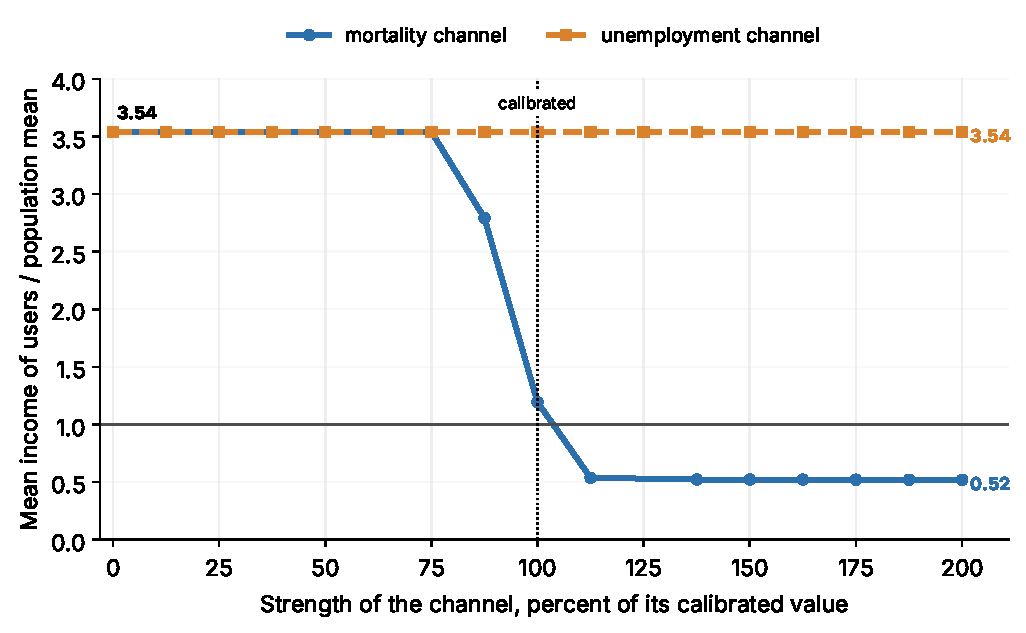
\includegraphics[width=0.66\textwidth]{figures/stylized_who_uses.pdf}
\caption{What it takes to reverse the income gradient in drug use}
\label{fig:who}
\notes{0.66\textwidth}{Note: the vertical axis is average income of users over the
population average, on a log scale, and $b$ is recalibrated at every point so
that participation is $5.13$ per cent throughout.}
\end{figure}

The result is sharper than the statement that mortality matters more. That
channel reverses the gradient at half of its calibrated strength, taking the
income ratio from $3.37$ to $0.19$, and does not move again; the unemployment
channel does not reverse it at all, leaving users at $3.37$ times average income
even fully switched on. A resource penalty \emph{cannot} produce the
concentration of drug use at the bottom, however strong it is made.

The asymmetry is not obvious, and the same logic operates in the quantitative
model. A resource penalty scales with the very thing it is meant to offset:
taking a fixed share of a large income still leaves a large income, so it cannot
outrun the fact that drugs are cheaper in utility terms for the rich. A
mortality penalty is different in kind, because what it destroys is not
resources but a continuation value, and the continuation value rises with
permanent income. The household with more to lose loses more, and loses
proportionally more than it gains from drugs being relatively cheap. This is why
$\aleph$ appears in equation~\eqref{eq:u}: it is the part of the continuation
value that does not shrink as consumption falls. The same channel carries the
policy result of Section~\ref{sec:mh}. Switch mortality off and the deterrent
effect of a universal voucher falls from $-3.00$ percentage points to $-0.37$,
which is to say it disappears: a voucher deters nobody once what drug use
threatens is only resources, because resources are what the voucher supplies
either way.

%======================================================================
\section{What housing assistance does}\label{sec:mh}

The two forces of question 2 can be separated exactly, because they differ in
what happens on acquiring the disorder. Under Treatment First the voucher is
withdrawn at that point, so only the value of life force operates; under
Housing First it is not, so both do. Comparing the two policies at the same
generosity therefore isolates the moral hazard, and comparing Treatment First
with no programme at all isolates the value of life.

\begin{figure}[!tb]
\centering
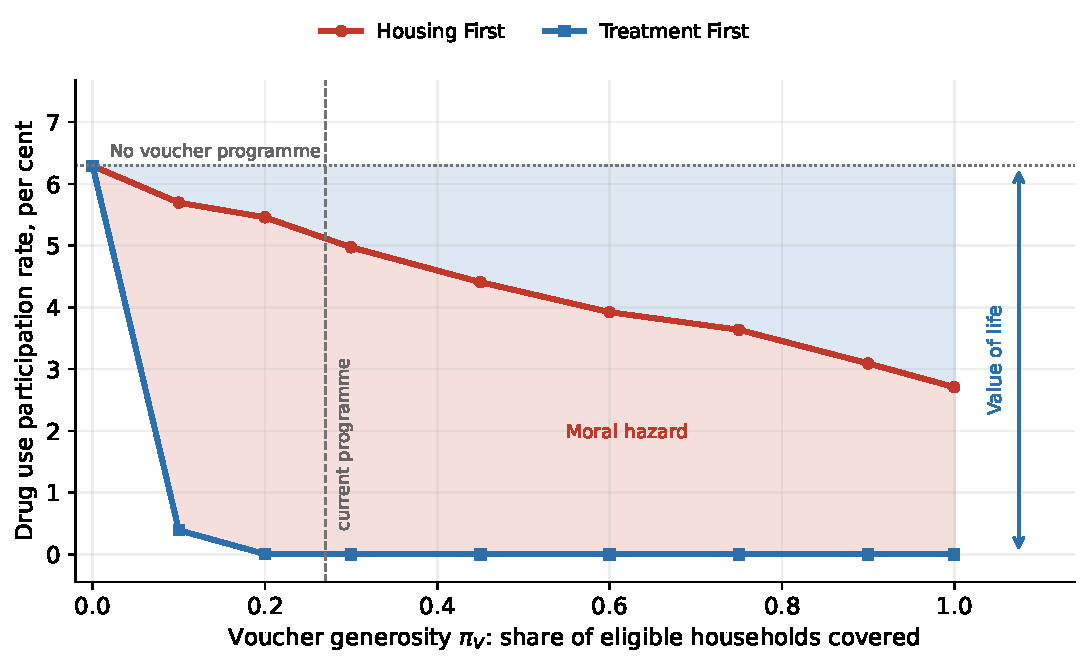
\includegraphics[width=0.70\textwidth]{figures/stylized_moral_hazard.pdf}
\caption{Drug use under the two policies as the voucher becomes more generous}
\label{fig:mh}
\notes{0.70\textwidth}{Note: the red band is the moral hazard and the blue band
above it is what Housing First delivers net; together they are the value of life
force, marked at the right. The dashed line is the current programme,
$\pi_V = 0.27$.}
\end{figure}

Figure~\ref{fig:mh} traces both as generosity rises. With no programme, $6.57$
per cent of households use. Universal Treatment First takes that to nothing, a value of life
force of $-6.57$ percentage points; universal Housing First leaves it at $3.57$
per cent, so the moral hazard is $+3.57$ points and the net effect of Housing
First is $-3.00$. Both forces are first order and they work against each other,
which is the central feature of the problem. Anyone asserting that housing the
homeless must increase drug use, or must reduce it, is making a quantitative
claim while sounding as though they are making a theoretical one.

Drug use is not what a housing programme is for, and a reader shown only
Figure~\ref{fig:mh} could conclude Treatment First wins on every count.
Figure~\ref{fig:margins} plots the outcomes the programme is aimed at alongside
drug use. On homelessness the two policies end in the same place, both driving it
from $0.63$ per cent to zero, with a gap along the way never exceeding a ninth of
a point. The difference is on the other margin, where at universal cover Housing
First leaves $0.63$ per cent of the population carrying the disorder and
Treatment First leaves none: the moral hazard shows up as disorder cases among
households who are housed, not as families left on the street.

\begin{figure}[!tb]
\centering
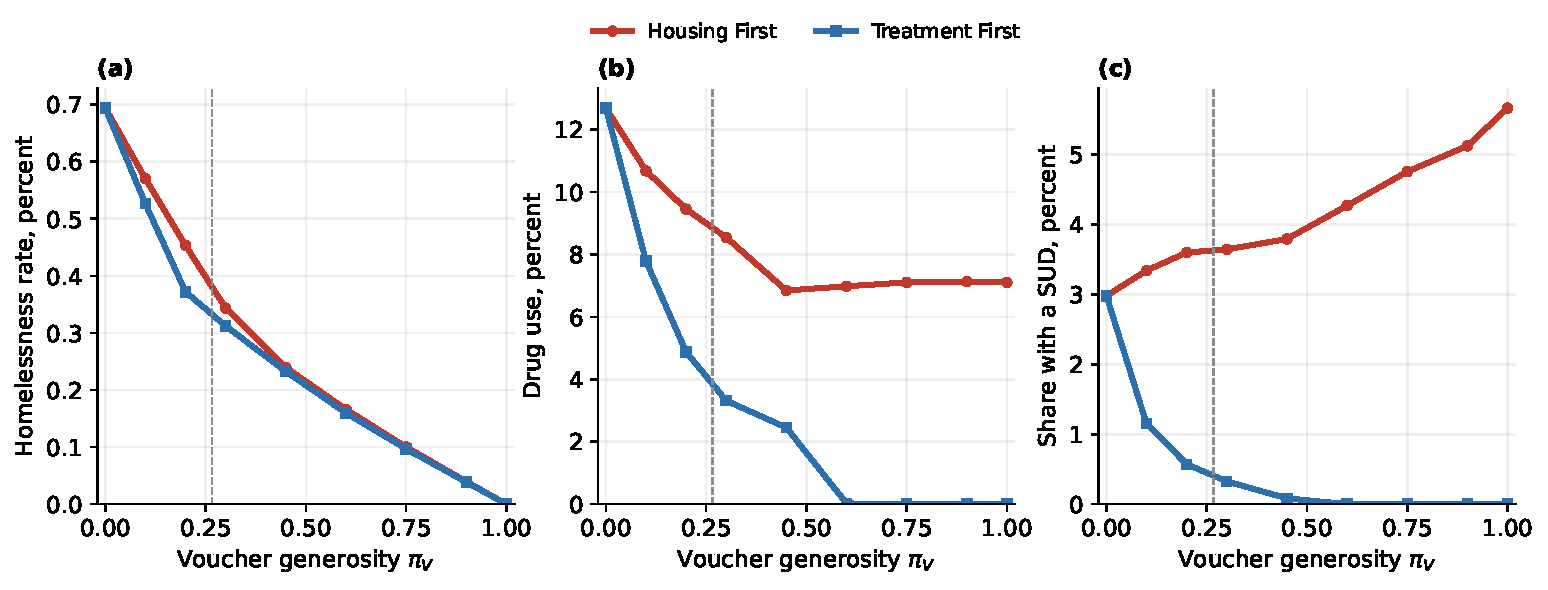
\includegraphics[width=1.0\textwidth]{figures/stylized_margins.pdf}
\caption{Homelessness, drug use and the disorder under the two policies}
\label{fig:margins}
\end{figure}

%======================================================================
\section{Welfare}\label{sec:welfare}

\subsection{Without externalities, Housing First always wins}\label{sec:nox}

Compare the policies at the same $\pi_V$. They differ only in the last indicator
in equation~\eqref{eq:vouch}, so Housing First transfers resources in a superset
of the states in which Treatment First does. The budget set is weakly larger in
every state and strictly larger in one, so a household that optimises cannot be
worse off:
\begin{equation}\label{eq:dom}
V_1(y;\ \text{HF},\ \pi_V) \;\ge\; V_1(y;\ \text{TF},\ \pi_V)
\qquad \text{for every } y,
\end{equation}
with equality exactly for households that never use. Put the other way round, a
household under Housing First can reproduce its Treatment First outcome exactly,
by not using. Conditionality removes an option from a forward looking optimiser
and gives nothing back. This is a dominance argument, not a calibrated result,
and no choice of parameters overturns it.

It follows that the moral hazard is not a distortion. Households here face the
true addiction hazard and make no mistakes, so the extra use Housing First
induces is not a wedge to be closed but a household taking a risk it is now
better able to bear, as an insured household drives in worse weather. The
$+3.57$ points of Section~\ref{sec:mh} is a statement about drug use and, on its
own, none about welfare. Table~\ref{tab:welfare} puts numbers on it: $4.1$ per
cent of households are strictly worse off under Treatment First, none is better
off, and those affected lose $0.39$ per cent of consumption.

\begin{table}[!tb]
\centering
\caption{Welfare at universal cover, with no externality}\label{tab:welfare}
\small
\begin{tabular}{@{}lcc@{}}
\toprule
& Housing First & Treatment First \\
\midrule
\multicolumn{3}{@{}l}{\emph{Panel A. Outcomes at universal cover}} \\
\quad Drug participation rate & 9.21\% & 0.00\% \\
\quad Share with a SUD & 9.209\% & 0.000\% \\
\quad Homelessness rate & 0.000\% & 0.000\% \\
\quad Voucher outlay per household & 0.0858 & 0.0851 \\
\addlinespace
\multicolumn{3}{@{}l}{\emph{Panel B. Treatment First against Housing First, no externality}} \\
\quad Households strictly worse off & & 10.1\% \\
\quad Households strictly better off & & 0.0\% \\
\quad Consumption equivalent, those affected & & 0.62\% \\
\quad Consumption equivalent, whole population & & 0.063\% \\
\bottomrule
\end{tabular}

\notes{0.9\textwidth}{Note: the consumption equivalent is the proportional change
in consumption, in every period and state, worth as much as the difference in
lifetime value. Voucher outlay is expected spending on a household from period 2
on, discounted, per unit of average income.}
\end{table}

A fixed budget does not rescue conditionality either. Treatment First is
slightly \emph{more} expensive at universal cover, $0.1833$ against $0.1830$, so
matching on cost rather than on generosity changes nothing. The reason is
unattractive and true: survival to period 3 falls from $0.93$ to $0.51$ with the
disorder, so the households the moral hazard adds to the rolls die sooner and
stop costing money.

So a case for conditionality must come from outside the model as it stands.
Households make no mistakes, so there is no internality; the policies cost the
same, so there is no fiscal argument; and drug use here touches nobody but the
user. The last is the one that can be measured rather than assumed, and the
table says in advance how large it must be: conditionality prevents $0.635$
percentage points of disorder cases at a private cost of $0.044$ per cent of one
lifetime income, so a social cost of $0.069$ of a lifetime income per case would
be exactly enough to justify it.

\subsection{The externality on children reverses it}\label{sec:kids}

\begin{table}[!tb]
\centering
\caption{The externality on children}\label{tab:children}
\footnotesize
\begin{tabular}{@{}lcccc@{}}
\toprule
\multicolumn{5}{@{}l}{\emph{Panel A. Transmission: what each income penalty implies}} \\
$\delta_d$ &  & Child's SUD rate & Ratio & CEV \\
\midrule
0.00 &  & \textcolor{red}{6.06\%} & 1.00 & 0.0\% \\
0.20 &  & \textcolor{red}{8.94\%} & \textcolor{red}{1.47} & 41.2\% \\
0.54\ \ (calibrated) &  & \textcolor{red}{18.19\%} & \textcolor{red}{3.00} & \textcolor{red}{216.5\%} \\
0.60 &  & \textcolor{red}{20.92\%} & \textcolor{red}{3.45} & \textcolor{red}{280.8\%} \\
\addlinespace
\multicolumn{5}{@{}l}{\emph{Panel B. Does the externality reverse the ranking?}} \\
\quad Private cost of conditionality &  &  &  & \textcolor{red}{0.090\%} \\
\quad Disorder cases prevented &  &  &  & \textcolor{red}{7.624 pp} \\
\quad CEV to the child, one case &  &  &  & \textcolor{red}{202.6\%} \\
\quad Externality gain from conditionality &  &  &  & \textcolor{red}{15.446\%} \\
\quad Gain over loss &  &  &  & \textcolor{red}{170.9} \\
\bottomrule
\end{tabular}

\notes{0.9\textwidth}{Note: Panel A is computed at the baseline programme,
$\pi_V=0.27$, since the transmission ratio in the data comes from an economy with
a rationed programme; loss to the child is its consumption equivalent loss per
lifetime income. Panel B is at universal cover, one child per household, no
discounting across generations.}
\end{table}

The link from a parent's addiction to a child has to run through income rather
than through preferences. Letting the child of a user inherit a stronger taste,
a lower $b$, matches the transmission fact but has the wrong welfare sign: $b$
enters only through $\theta\log(1+v/b)$, so a lower one raises the child's
objective at every $v>0$ and its lifetime value with it. Letting it inherit a
greater susceptibility, a higher $\lambda$, fails the other way, since a child
facing a riskier drug uses \emph{less}. Income works on both counts, and it
works because of Section~\ref{sec:who}: lower permanent income is unambiguously
bad to receive, and this model already puts users at the bottom, so a child born
poorer is mechanically more likely to use. The income gradient does the whole
job, so the model transmits addiction across generations \emph{without
transmitting any preference for drugs}. A child's baseline income is drawn from
the same lognormal as everyone else, and the entire link is the penalty
\begin{equation}\label{eq:kids}
y_{\text{child}} \;=\; y_{\text{base}}\,
(1-\delta_d)^{\mathbf{1}\{\text{parent acquired the disorder}\}}\,
(1-\delta_h)^{\mathbf{1}\{\text{parent was homeless}\}} ,
\end{equation}
which the parent does not internalise. That is what makes it an externality
rather than something already priced into $V_1$. General income persistence is
absent because it is not an externality: it operates whether or not the parent
uses.

The two penalties are set to different things. Panel A of
Table~\ref{tab:children} shows that $\delta_d = 0.30$ makes the child of a parent
who acquired the disorder $2.4$ times as likely to acquire one, in the middle of
the epidemiological range of two to four in McGovern et al.\ (2023) and the
alcohol literature. For $\delta_h$, Chetty, Hendren and Katz (2016) find children
moved to a low poverty neighbourhood before age 13 earned $31$ per cent more as
adults, which is conservative here since growing up homeless is presumably
worse. The two do different work: both policies drive homelessness to zero at
universal cover, so $\delta_h$ prices the programme against no programme while
$\delta_d$ decides Treatment First against Housing First.


Panel B puts the two sides together and they are not close. The private cost of
conditionality is $0.044$ per cent of a lifetime income, small because only $4.1$
per cent of households are affected. Against that, conditionality prevents
$0.635$ percentage points of disorder cases, and each costs one child $90$ per
cent of a lifetime income, far above the $6.9$ per cent threshold set out above.
The externality gain is thirteen times the private loss, and stays above it
throughout the range of $\delta_d$ in Panel A. Housing First is better for every
household taken one at a time, and worse once one counts the children of the
households it fails to deter.

Whether any of this is an externality at all depends on how much of it parents
already take into account, and the evidence points both ways. Substance use
falls sharply during pregnancy in the NSDUH and rises again afterwards, and
entry into treatment clusters around child welfare involvement, neither of which
fits a parent placing no weight on a child. Equally plainly the weight is not
one: parental drug use is recorded in roughly a third of foster care removals,
and Altonji, Hayashi and Kotlikoff (1992) reject full altruism outright. A pure
generational discount is a useful anchor for how much to allow, and at $\beta =
0.96$ over thirty years it is $0.29$. This is the assumption the case for
conditionality is most sensitive to, and the quantitative model treats it as
such, putting the child's value in the parent's own objective at a weight of
$25$ per cent rather than assuming the weight is zero.

\subsection{What this settles and what it does not}

One feature of the model inflates that margin, and it is the right note on which
to hand the question over. Treatment First drives drug use to \emph{exactly} zero
here, an artifact of having no preference heterogeneity: a policy strong enough
to deter the marginal user deters every one. Nobody faces the condition and
fails to meet it, and those households are the entire empirical case for Housing
First. Establishing which way each comparison goes, with them, a government
budget, an equilibrium drug price and a proper life cycle, is what the
quantitative model is for.

%======================================================================
\section*{References}
{\footnotesize\setlength{\parskip}{0em}\par
Chetty, R., N. Hendren and L. Katz (2016). ``The Effects of Exposure to Better
Neighborhoods on Children.'' \emph{AER} 106(4).\ \
Altonji, J., F. Hayashi and L. Kotlikoff (1992). ``Is the Extended Family
Altruistically Linked?'' \emph{AER} 82(5), 1177--98.\ \
Heathcote, J., F. Perri and G. Violante (2010). ``Unequal We Stand.'' \emph{RED}
13(1), 15--51.\ \
Hjorth\o j, C. et al.\ (2023). Excess mortality among people with substance use
disorders.\ \
McGovern, R. et al.\ (2023). ``Maternal and paternal substance use and child
substance use.'' \emph{Addiction} 118(5).\ \
Viscusi, W. K. and J. Aldy (2003). ``The Value of a Statistical Life.''
\emph{Journal of Risk and Uncertainty} 27(1), 5--76.\ \
Data: SAMHSA (NSDUH 2024, TEDS); HUD; BLS; ACS; CDC; DOL.\par}

\end{document}
